\documentclass[a4paper]{article}  
\usepackage{ctex}
\usepackage{graphicx}
\usepackage{geometry}
\usepackage{hyperref}
\usepackage{fancyhdr}  
\usepackage{float}
\usepackage{xcolor}  % 加载颜色包
\usepackage{listings}  % 加载listings包
\hypersetup{
colorlinks=true,
linkcolor=black
}
\geometry{left=2.5cm,right=2.5cm,top=2.5cm,bottom=2.5cm}

\pagestyle{fancy}                 
% 设置页眉页脚风格为 fancyhdr 提供的“fancy”模式
\fancyhf{}                        
% 清空默认的页眉页脚
\fancyhead[C]{系统开发工具基础 实验报告} 
% 页眉(head),C 表示居中,内容是标题
\fancyfoot[C]{\thepage}           
% 页脚(foot),C 表示居中,内容是页码 \thepage

\begin{document} 

\begin{titlepage}  
    \centering  
    \huge \textbf{《系统开发工具基础》实验报告}
    \vspace{5cm}  
    \begin{figure}[ht]
    \centering
    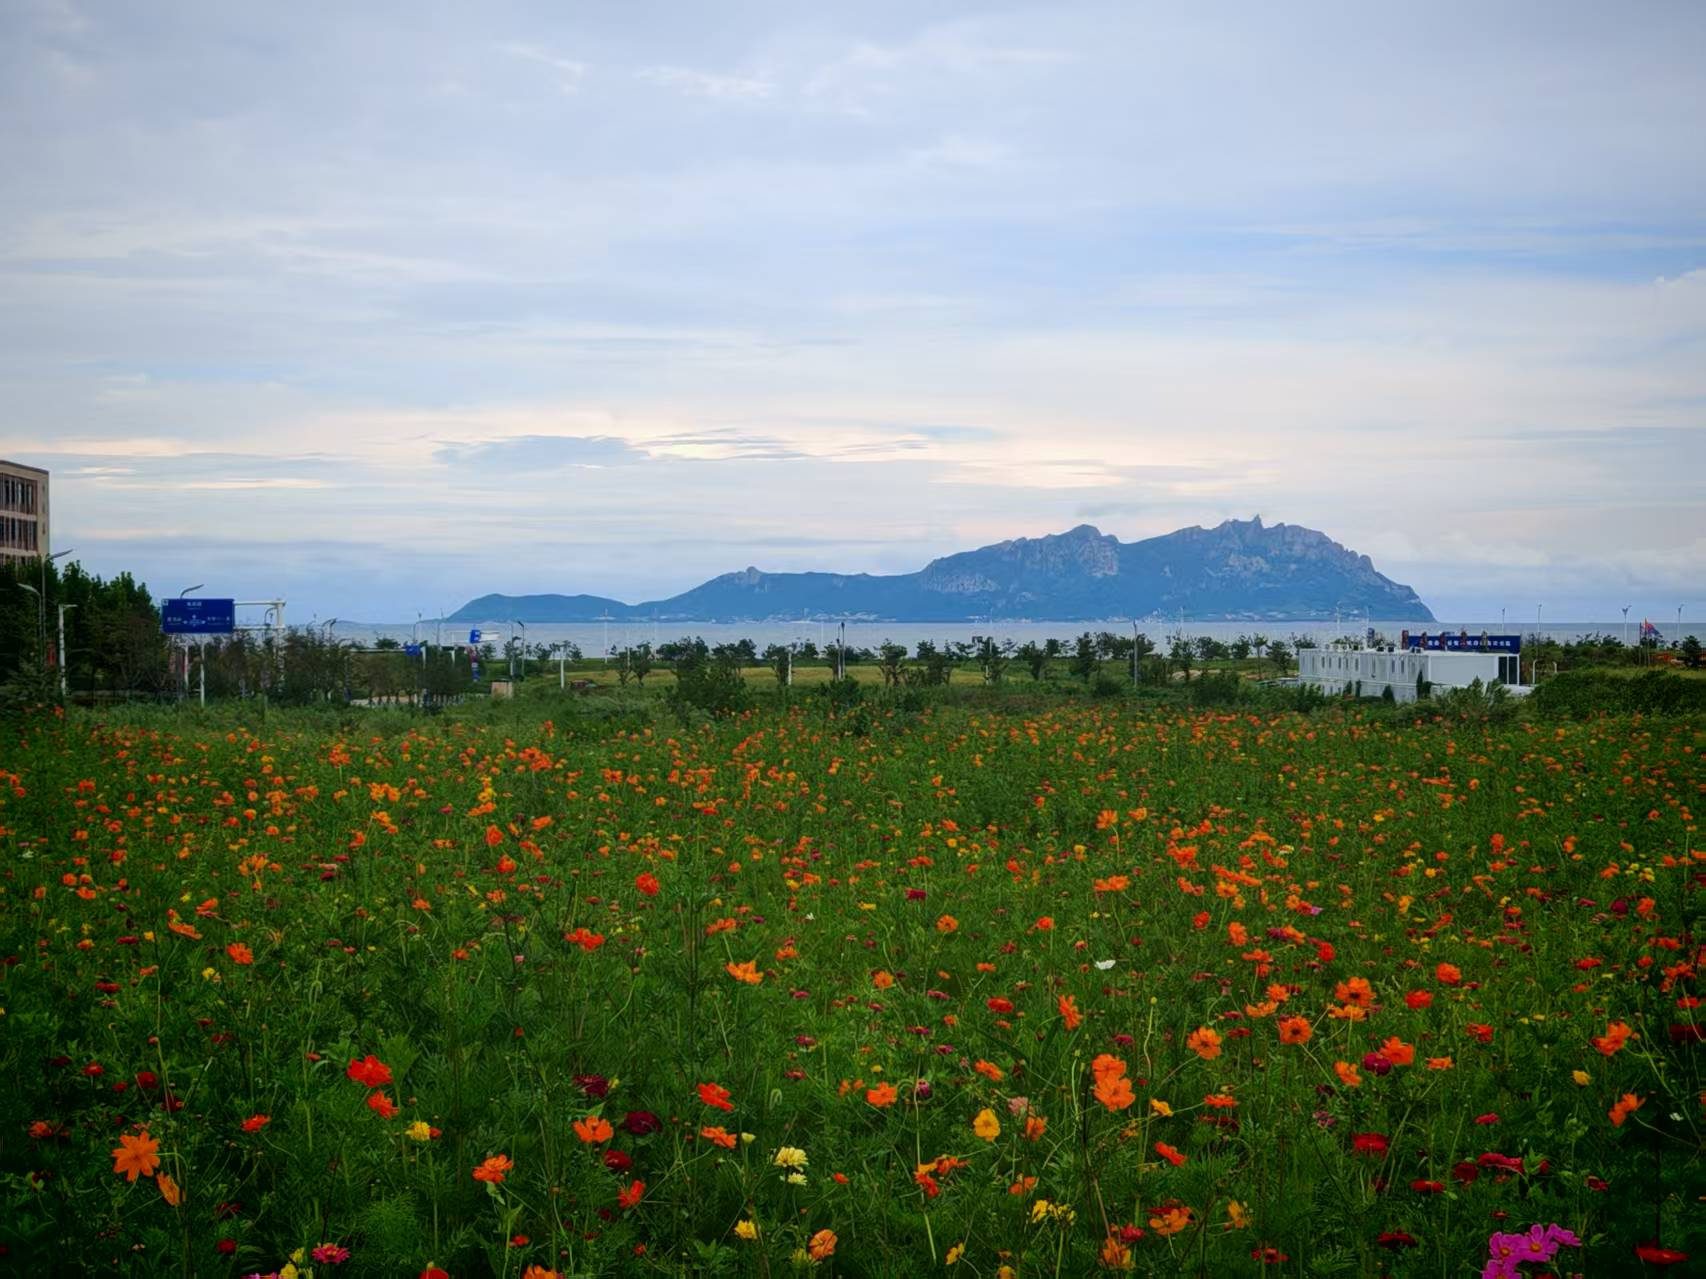
\includegraphics[width=0.6\textwidth]{images/face.jpg}
    \end{figure}
    
    \Large  
    \vspace{3cm} 
 
    \begin{tabular}{ll} 
        \textbf{主题:}& git + Latex\\
        \cline{2-2} 
        \textbf{学号:} & 24020007088 \\ 
       \cline{2-2} 
        \textbf{姓名:} & 马一诺 \\  
        \cline{2-2} 
        \textbf{专业:} & 计算机科学与技术 \\  
       \cline{2-2} 
       \textbf{我的github:} & \href{https://github.com/1-qaz-2-wsx/sys-dev-tools}{点击这里} \\
       \cline{2-2} 
    \end{tabular}  
    \vspace{2cm}  
 
    \Large 日期: \today  
    
\end{titlepage}  

\pagenumbering{roman}
\tableofcontents

\newpage
\pagenumbering{arabic}
\section{实验目的}  
1.了解并学习版本控制Git;

2.了解并学习Latex文本编辑;
\section{实验内容}
1.学习了Git的工作原理、基本操作、如何关联本地仓库和远程仓库。

2.学习了用LaTeX编写文档,并编写实验报告模板。

\section{实例}
\subsection{实例一:克隆课程网站的存储库}
    \begin{figure}[ht]
    \centering
    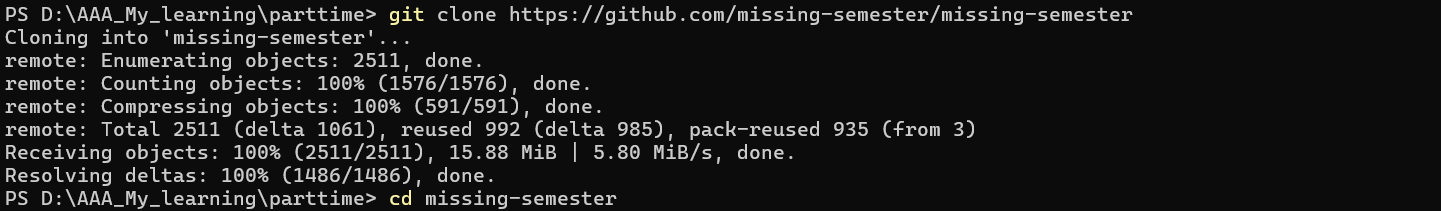
\includegraphics[width=1\textwidth]{images/clone.png}
    \caption{实例一:克隆课程网站的存储库}
    \label{fig:gitlog}
    \end{figure}
\subsection{实例二:尝试本地新建分支}
    \begin{figure}[ht]
    \centering
    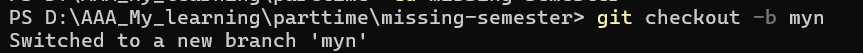
\includegraphics[width=1\textwidth]{images/checkout.png}
    \caption{实例二:尝试本地新建分支}
    \label{fig:checkout}
    \end{figure}

\subsection{实例三:log查看历史提交记录}

    \begin{figure}[H]
    \centering
    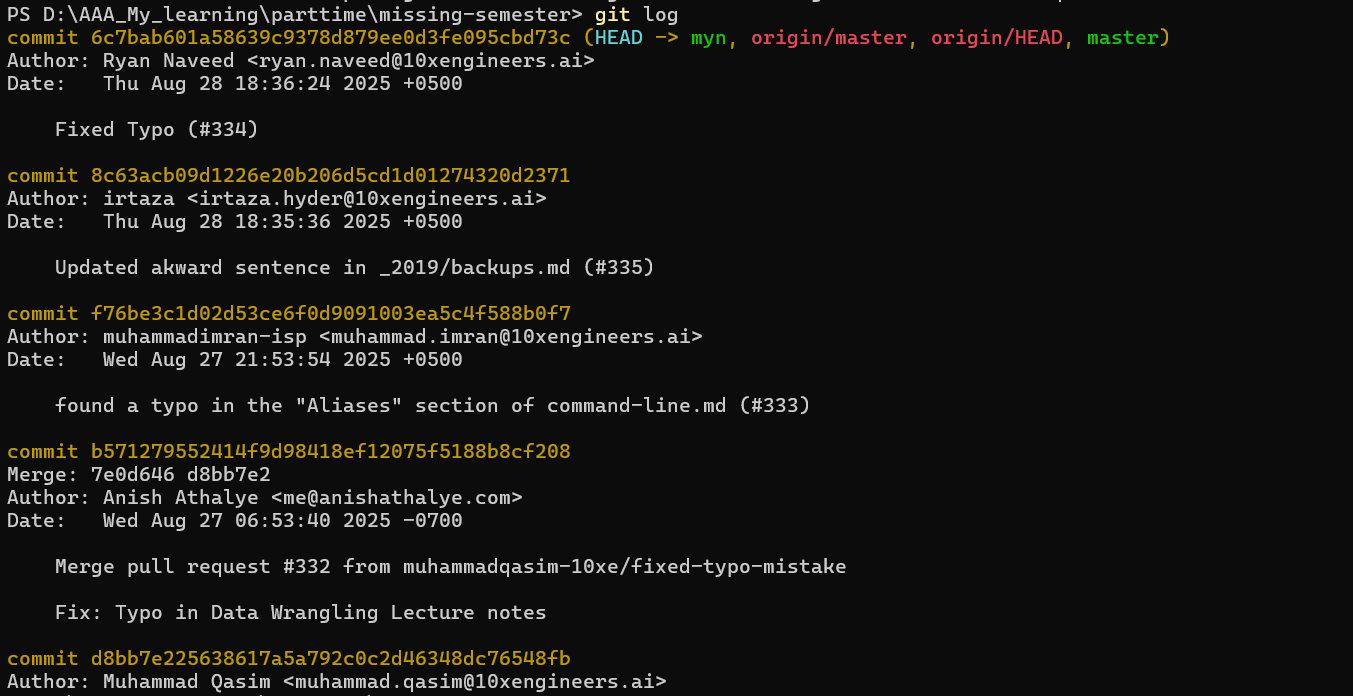
\includegraphics[width=1\textwidth]{images/log.png}
    \caption{log}
    \label{log}
    \vspace{1cm}
    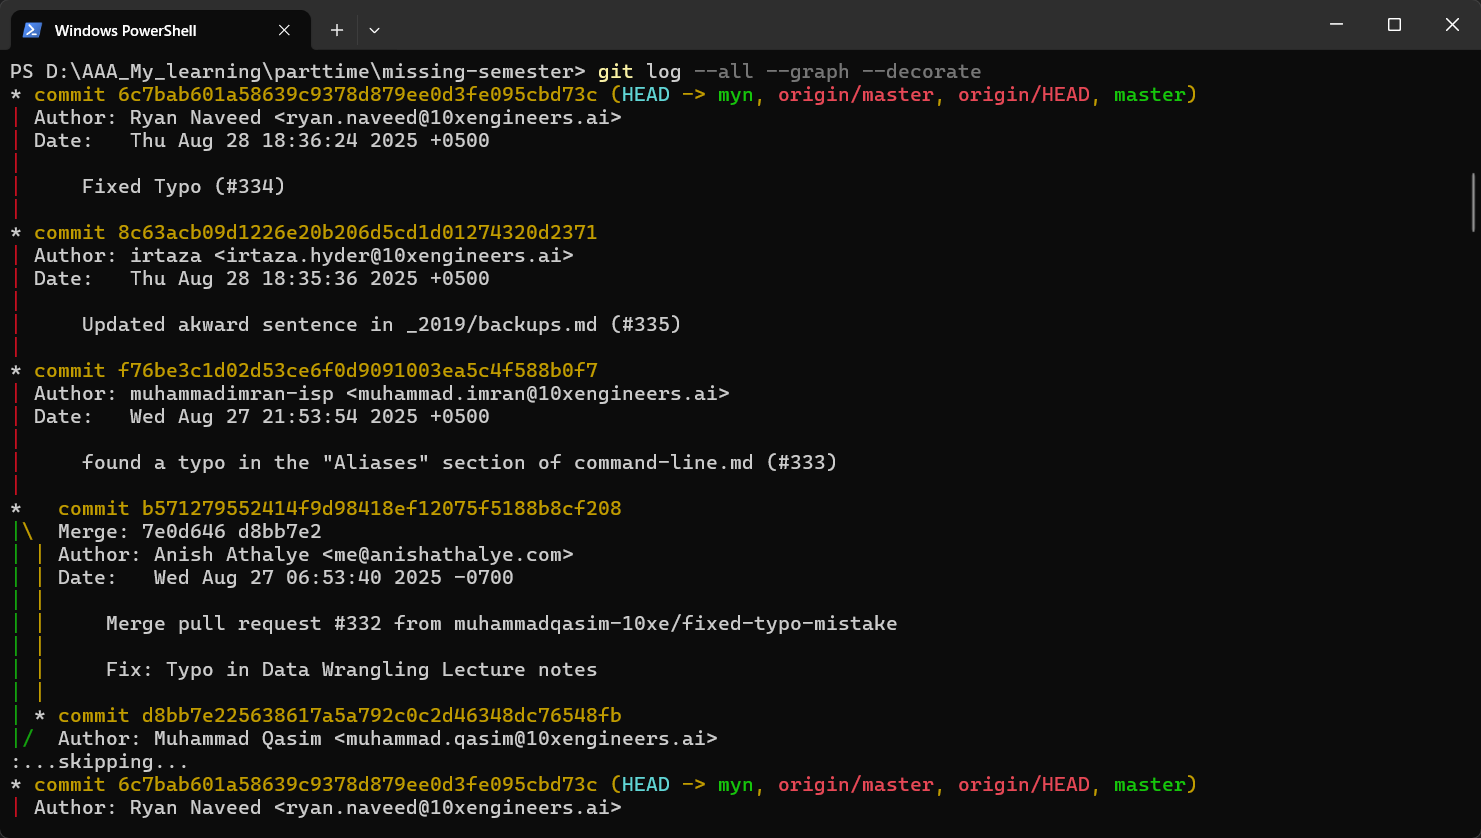
\includegraphics[width=1\textwidth]{images/log2.png}
    \caption{将历史记录可视化为DAG}

    \end{figure}

   

\subsection{实例四:最后一次修改 \_config.yml 文件中 collections: 行时的提交信息是什么?}

\begin{figure}[H]
    \centering
    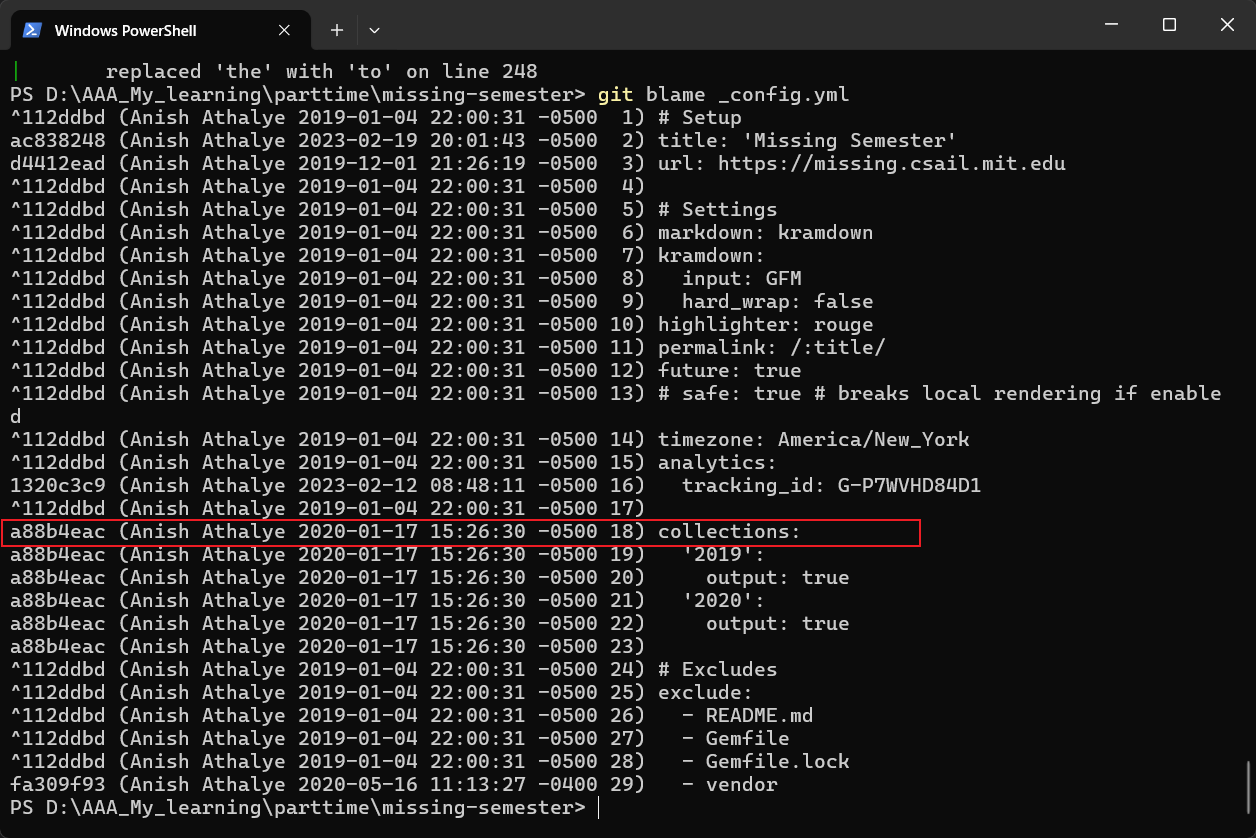
\includegraphics[width=1\textwidth]{images/blame.png}
    \caption{\texttt{git blame}:逐行显示文件最后一次修改的提交、作者、时间}
    \end{figure}
    \vspace{1cm}

    \begin{figure}[H]
    \centering
    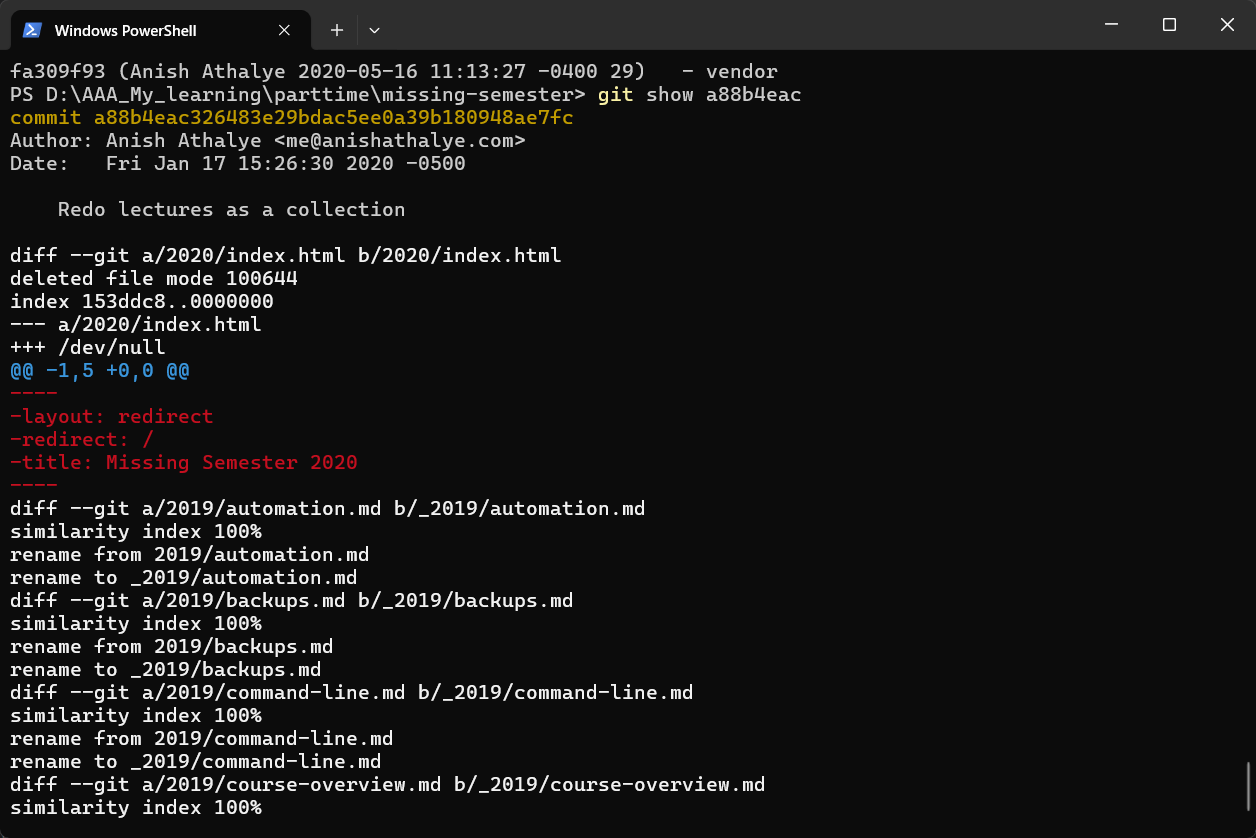
\includegraphics[width=1\textwidth]{images/show.png}
    \caption{\texttt{git show}:展示某个提交的详细信息(提交消息 + 修改内容)。}
    \end{figure}

\subsection{实例五:机密文件上传}
    \begin{figure}[H]
    \centering
    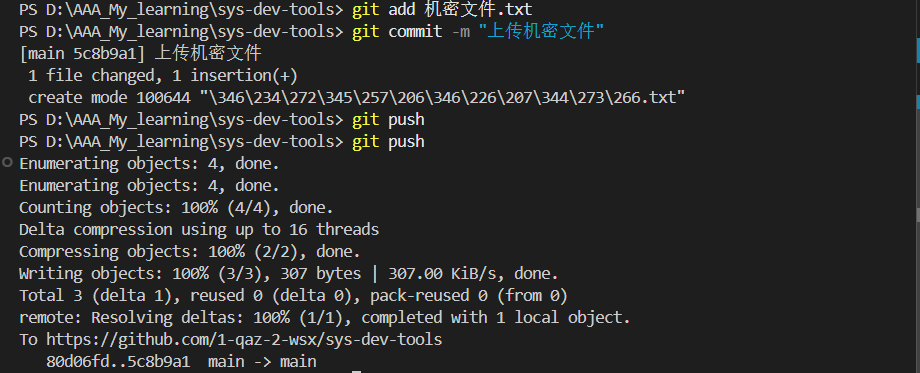
\includegraphics[width=1\textwidth]{images/addSecret.png}
    \caption{推送到远程仓库}
    \end{figure}
\subsection{实例六:如何删除敏感文件记录}
    \begin{figure}[H]
    \centering
    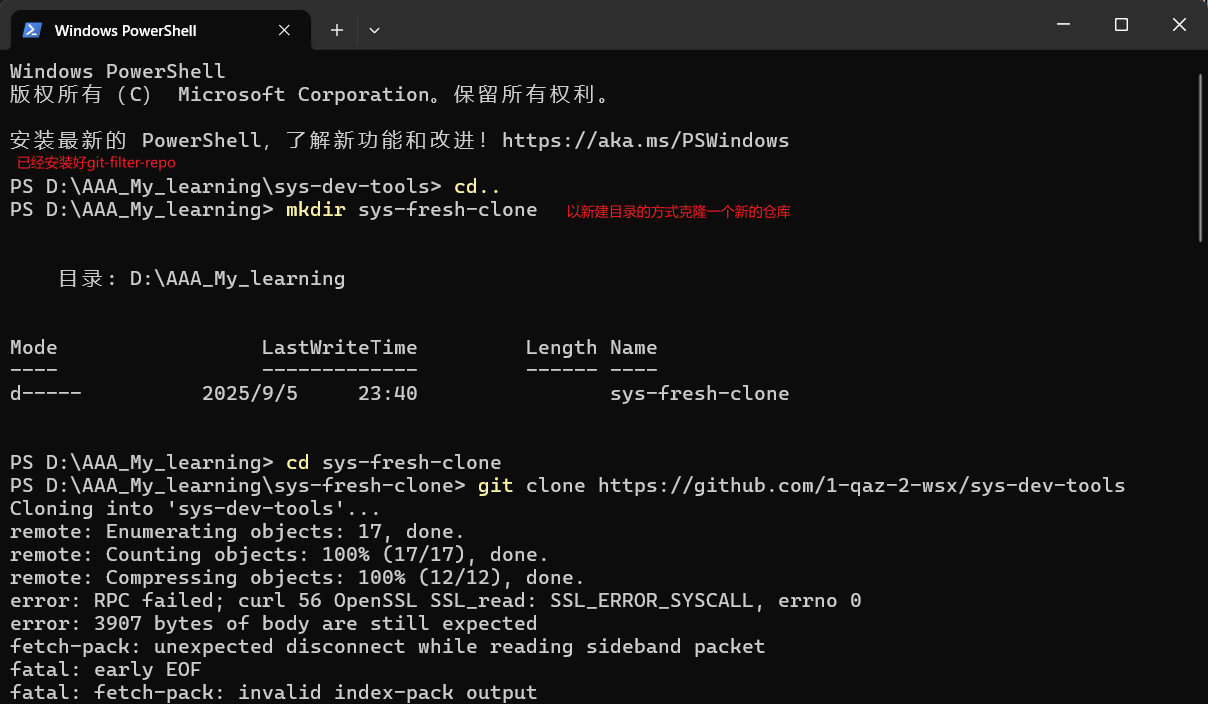
\includegraphics[width=1\textwidth]{images/delete1.png}
    \caption{delete1}
    \end{figure}
    \vspace{1cm}

        \begin{figure}[H]
    \centering
    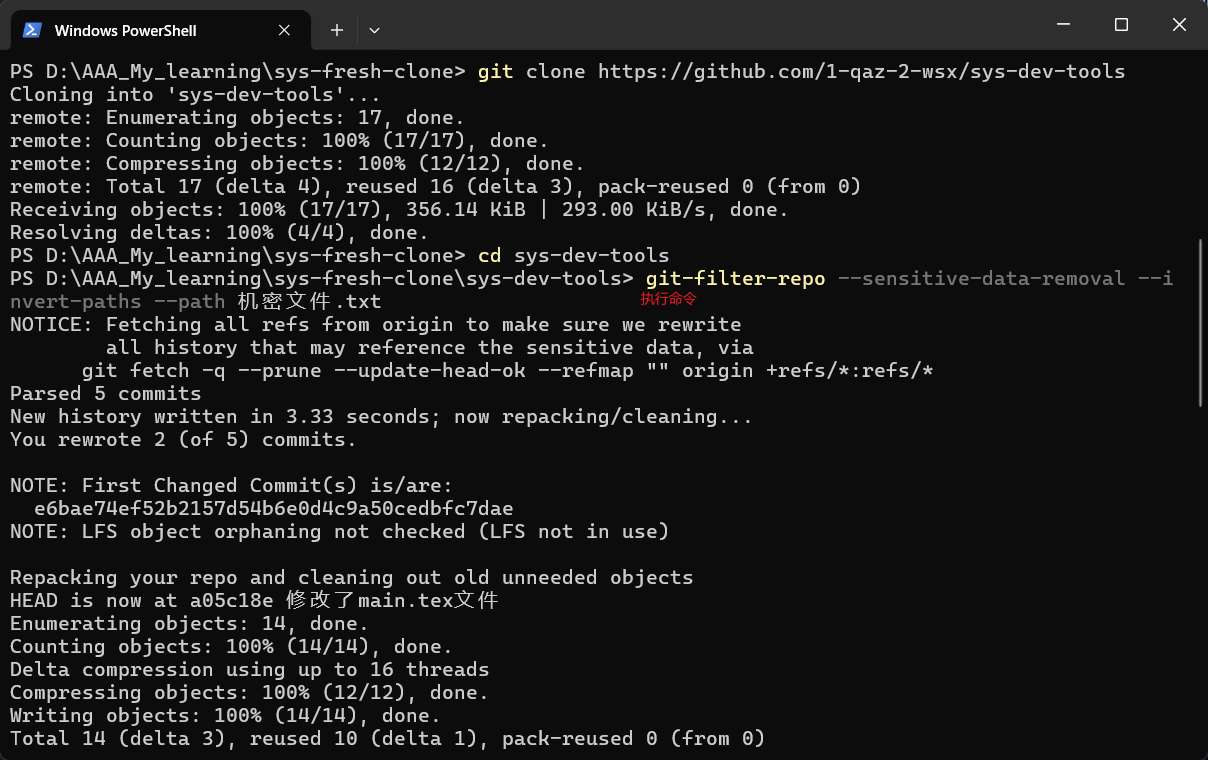
\includegraphics[width=1\textwidth]{images/delete2.png}
    \caption{delete2}
    \end{figure}
    \vspace{1cm}

        \begin{figure}[H]
    \centering
    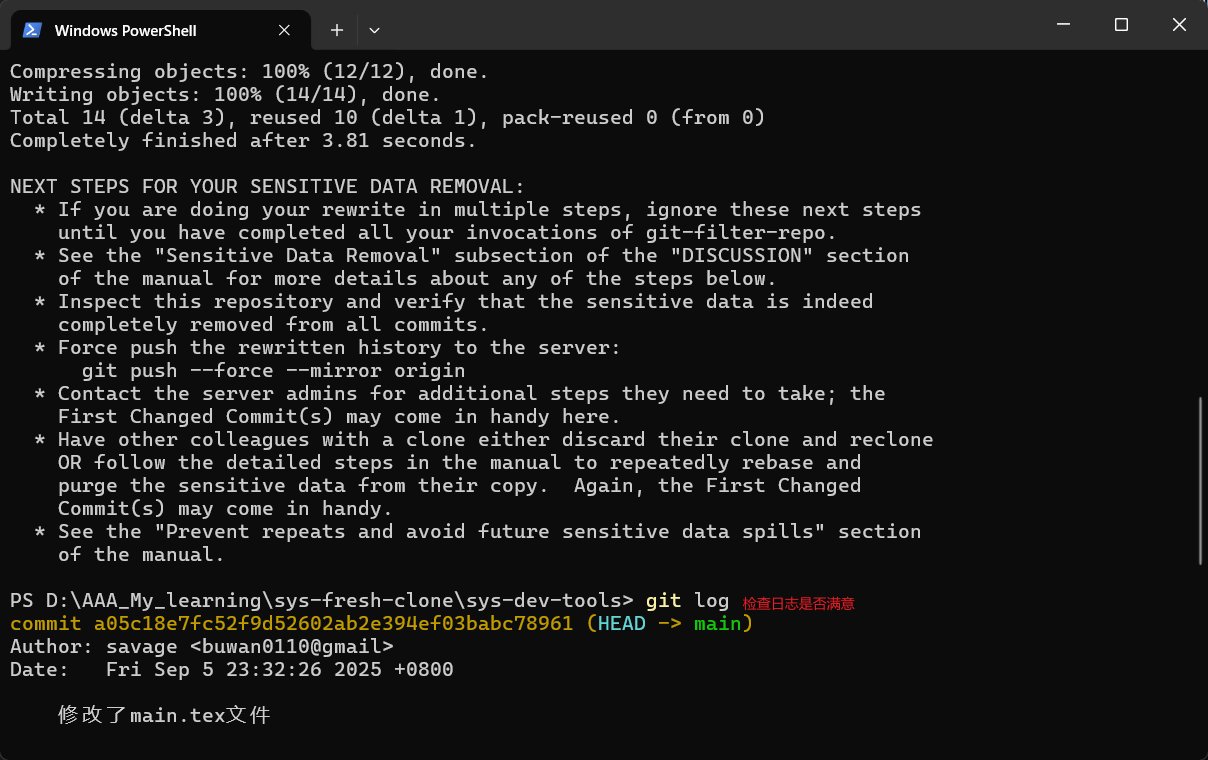
\includegraphics[width=1\textwidth]{images/delete3.png}
    \caption{delete3}
    \end{figure}
    \vspace{1cm}

        \begin{figure}[H]
    \centering
    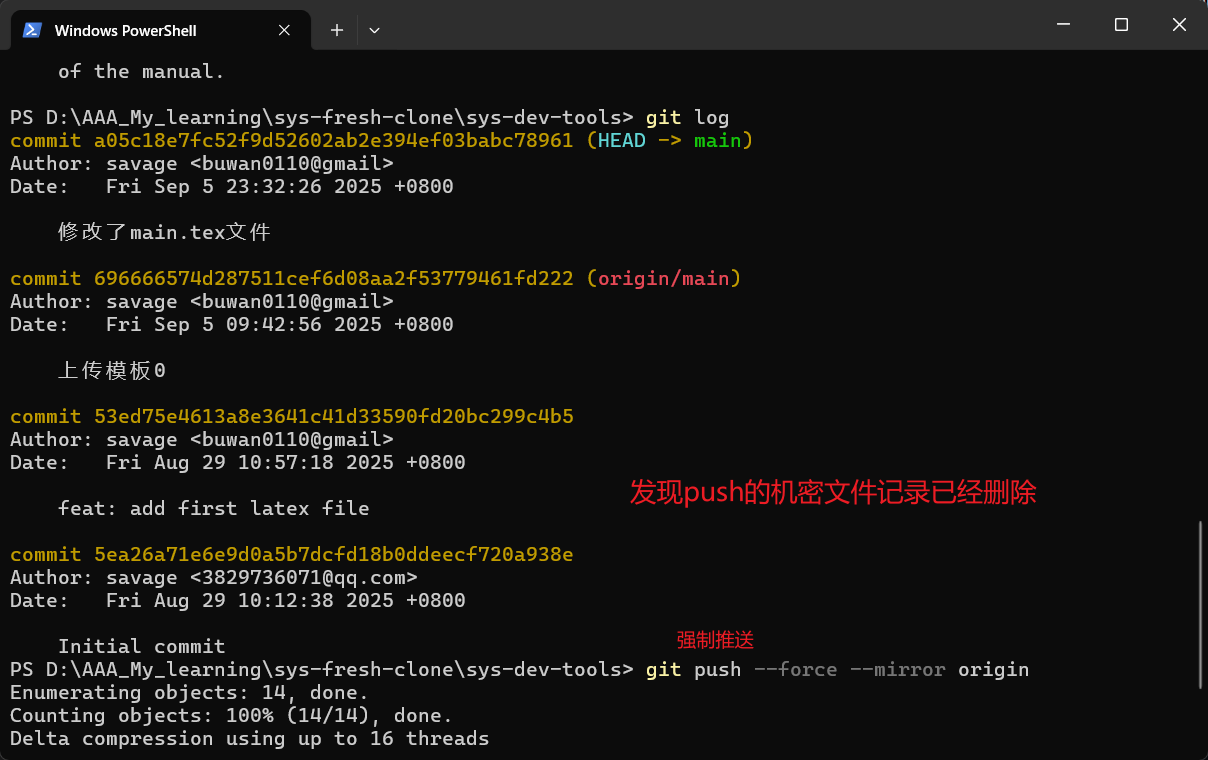
\includegraphics[width=1\textwidth]{images/delete4.png}
    \caption{delete4}
    \end{figure}

\subsection{实例七:使用stash(和add不同)}

    \begin{figure}[H]
    \centering
    
\includegraphics[width=1\textwidth]{images/stash.png}
    \caption{\texttt{git stash}}
    \end{figure}
    已经把当前未提交的修改保存成一个临时快照(stash),标记为 WIP on main。

    当需要暂时保存但又不提交时,使用\texttt{git stash}将改动存放到特殊的栈里,后续需要commit时再pop(实例八)
\subsection{实例八:stash后的提交记录以及弹出stash}
    \begin{figure}[H]
    \centering
    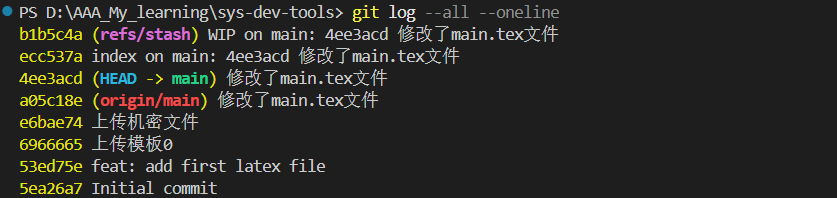
\includegraphics[width=1\textwidth]{images/stash-log.png}
    \caption{stash-log}
    \end{figure}
        \begin{figure}[H]
    \centering
    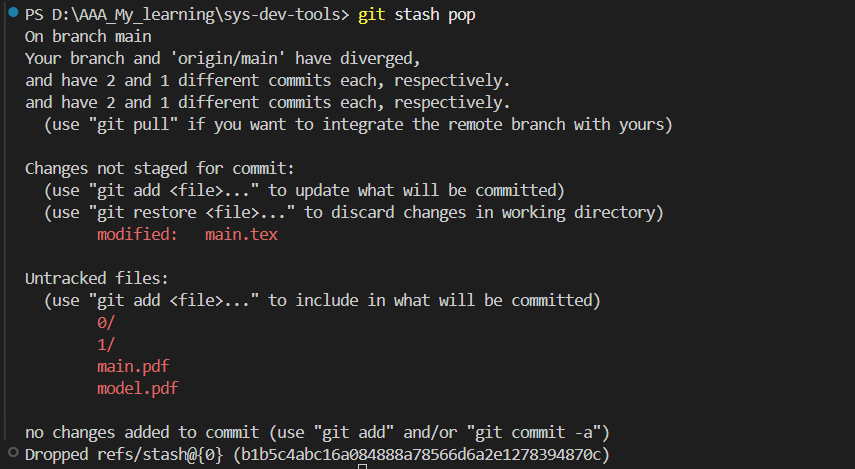
\includegraphics[width=1\textwidth]{images/pop.png}
    \caption{pop}
    \end{figure}

\subsection{实例九:为长命令设置别名}
    \begin{figure}[H]
    \centering
    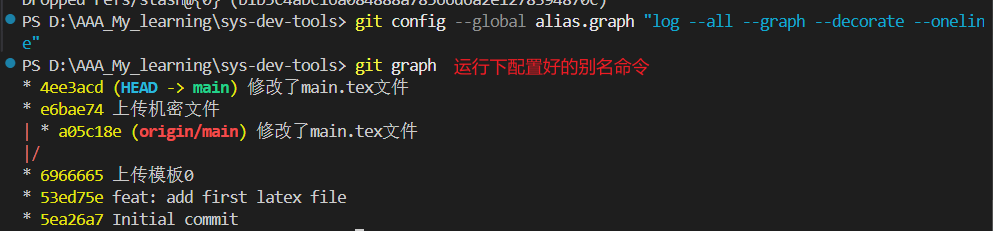
\includegraphics[width=1\textwidth]{images/graph.png}
    \caption{alias}
    \end{figure}

\subsection{实例十:全局忽略规则}
已经在新建仓库时初始化好,忽略跟踪临时文件,可以看到github仓库没有临时文件的上传
    \begin{figure}[H]
    \centering
    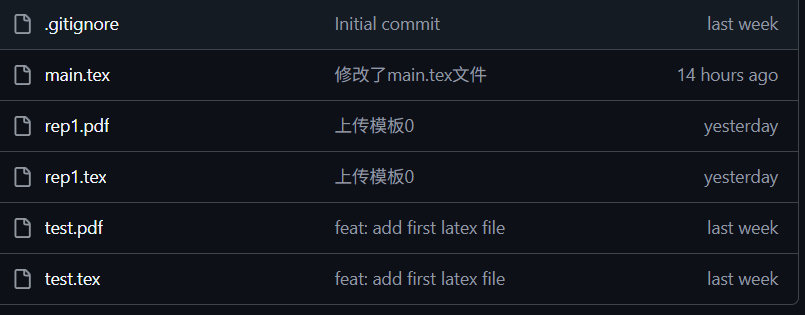
\includegraphics[width=1\textwidth]{images/ignore1.png}
    \caption{ignore1}
    \end{figure}
检查仓库状态,确定没有追踪不必要的临时文件
        \begin{figure}[H]
    \centering
    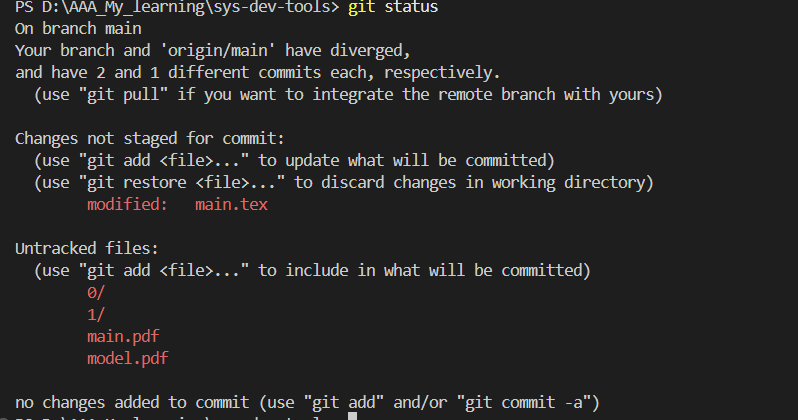
\includegraphics[width=1\textwidth]{images/ignore2.png}
    \caption{ignore2}
    \end{figure}
\subsection{实例十一:推送分支、合并分支}
    \begin{figure}[H]
    \centering
    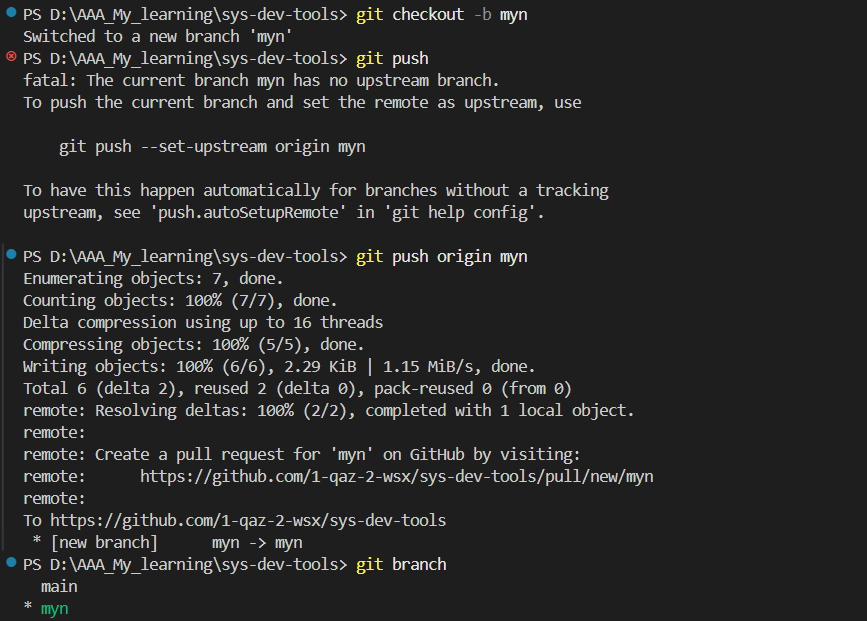
\includegraphics[width=1\textwidth]{images/branch1.png}
    \caption{branch1}
    \end{figure}

    \begin{figure}[H]
    \centering
    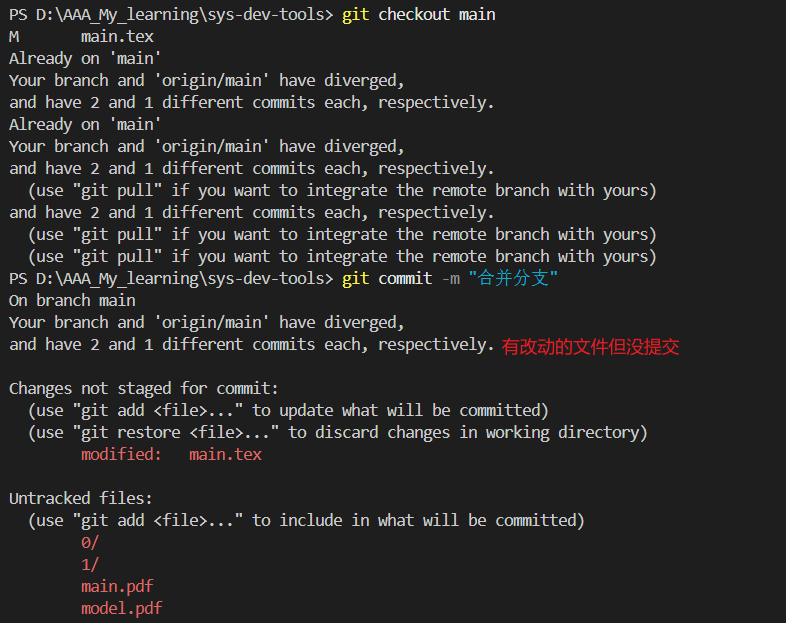
\includegraphics[width=1\textwidth]{images/branch2.png}
    \caption{branch2}
    \end{figure}

    \begin{figure}[H]
    \centering
    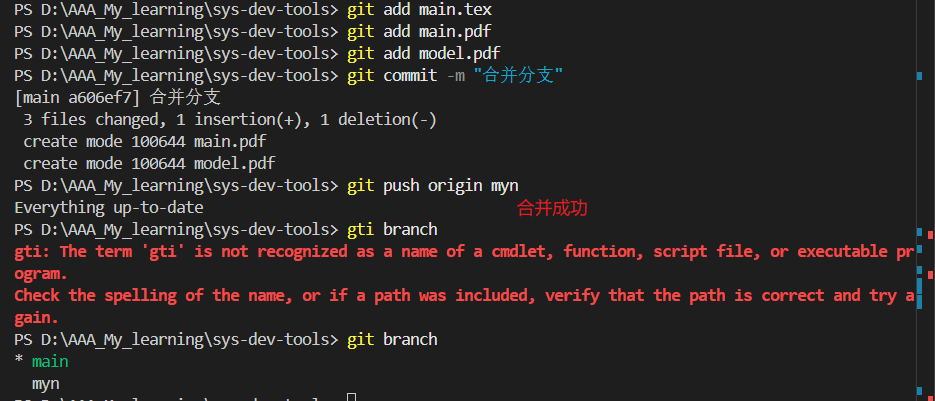
\includegraphics[width=1\textwidth]{images/branch3.png}
    \caption{branch3}
    \end{figure}    
\subsection{实例十二:删除本地和远程分支}
如果确定已经合并好分支并且不需要分分支时,可以对分支进行删除
    \begin{figure}[H]
    \centering
    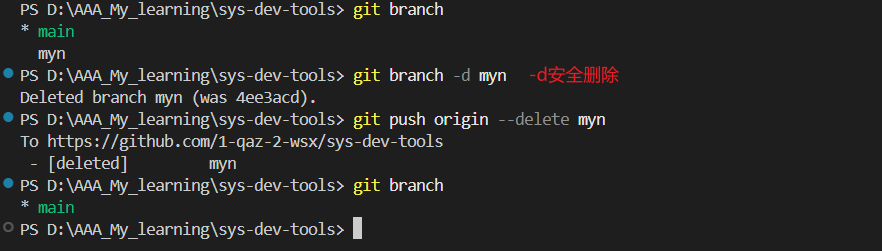
\includegraphics[width=1\textwidth]{images/dBranch.png}
    \caption{delete branch}
    \end{figure}
\subsection{实例十三:git diff查看工作区和暂存区间的差异}
    
    \begin{figure}[H]
    \centering
    
\includegraphics[width=1\textwidth]{images/diff1.png}
    \caption{diff1}
    \end{figure}
    \begin{figure}[H]
    \centering
    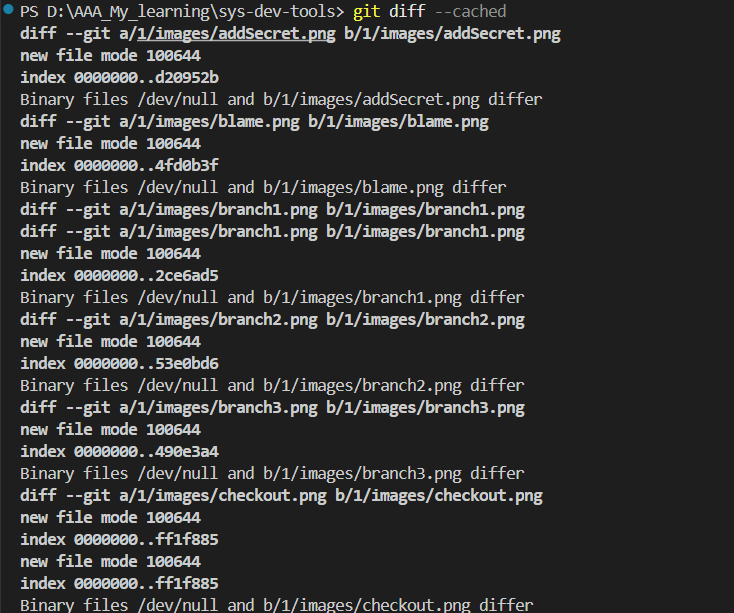
\includegraphics[width=1\textwidth]{images/diff2.png}
    \caption{diff2}
    \end{figure}

\subsection{实例十四:Latex插入图片}
    \begin{figure}[H]
    \centering
    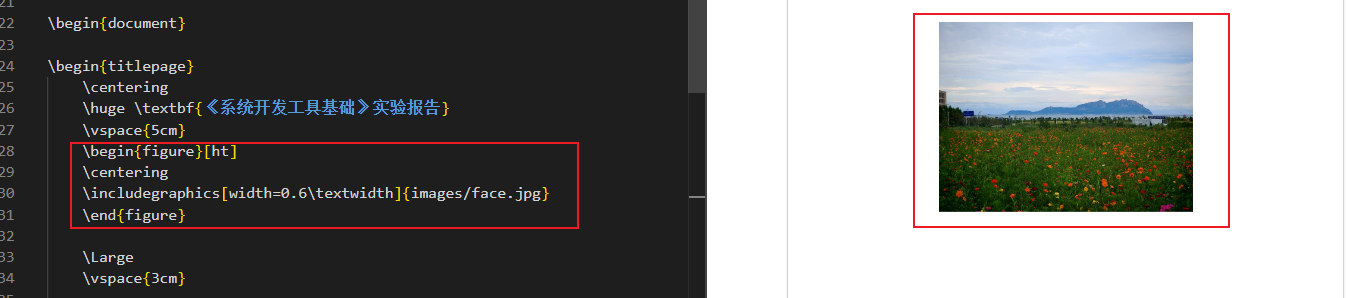
\includegraphics[width=1\textwidth]{images/insertGraph.png}
    \caption{insert graph}
    \end{figure}
\subsection{实例十五:Latex解决图片排版乱跑}
    \begin{figure}[H]
    \centering
    
\includegraphics[width=1\textwidth]{images/force1.png}
    \caption{force1}
    \end{figure}
    \begin{figure}[H]
    \centering
    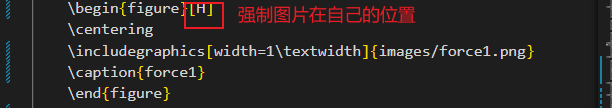
\includegraphics[width=1\textwidth]{images/force2.png}
    \caption{force2}
    \end{figure}

\subsection{实例十六:添加目录}
    \begin{figure}[H]
    \centering
    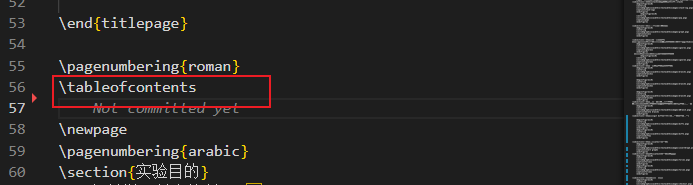
\includegraphics[width=1\textwidth]{images/tableofcontents.png}
    \caption{tableofcontents}
    \end{figure}
\subsection{实例十七:添加页眉页脚}
    \begin{figure}[H]
    \centering
    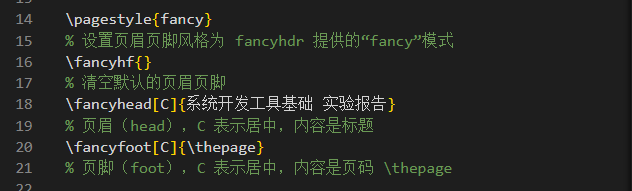
\includegraphics[width=1\textwidth]{images/headFoot.png}
    \caption{headFoot}
    \end{figure}
\subsection{实例十八:插入代码块}

\lstset{
 columns=fixed,       
 numbers=left,                                       
 numberstyle=\tiny\color{gray},                      
 frame=none,                                         
 backgroundcolor=\color[RGB]{245,245,244},           
 keywordstyle=\color{blue},    
 stringstyle=\rmfamily\color[RGB]{128,0,0},
 language=c++,                                      
}
\begin{lstlisting}

#include <iostream>
using namespace std;

int main()
{
    cout<<"hello"<<endl;
    return 0;
}
\end{lstlisting}

代码如图\ref{code}
    \begin{figure}[H]
    \centering
    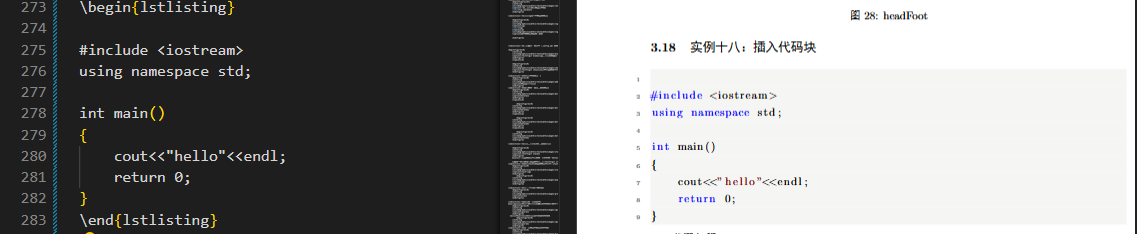
\includegraphics[width=1\textwidth]{images/code.png}
    \caption{code}
    \label{code}
    \end{figure}
\subsection{实例十九:插入链接}
如图\ref{link}
    \begin{figure}[H]
    \centering
    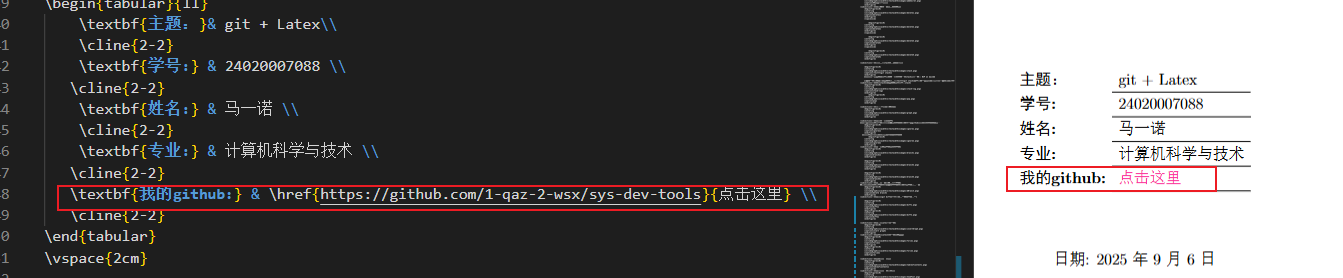
\includegraphics[width=1\textwidth]{images/link.png}
    \caption{link}
    \label{link}
    \end{figure}
\subsection{实例二十:插入公式}

\begin{eqnarray}
     e&=&mc^2 \\
     \pi&=&\frac{c}{d}\\
     \frac{d}{dx}\int_0^{\infty} f(s)ds&=&f(s)\\
     f(x)&=&\sum_{i} 0^{\infty}\frac{f^{(i)}(0)}{i!}x^i \\
     x&=&\sqrt{\frac{x_i}{z}y}
\end{eqnarray}

    \begin{figure}[H]
    \centering
    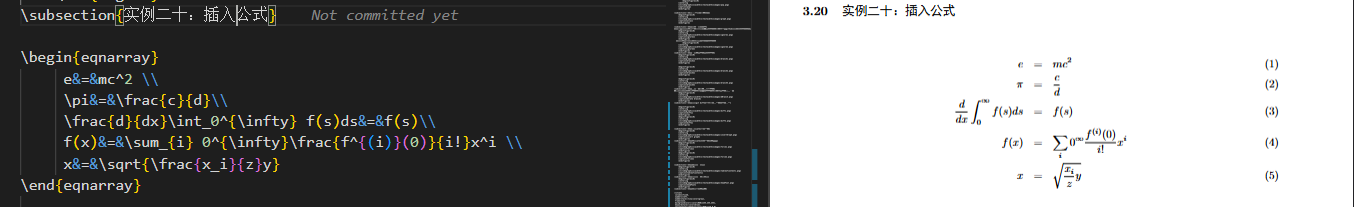
\includegraphics[width=1\textwidth]{images/enq.png}
    \caption{eqnarray}
    \end{figure}
\section{实验结果}

\subsection{git}
了解学习了git的基本操作,创建了自己的远程github仓库并与本地仓库关联。

了解学习了latex的基本操作,创建了实验报告模板。如图\ref{model1}和\ref{model2}
    \begin{figure}[H]
    \centering
    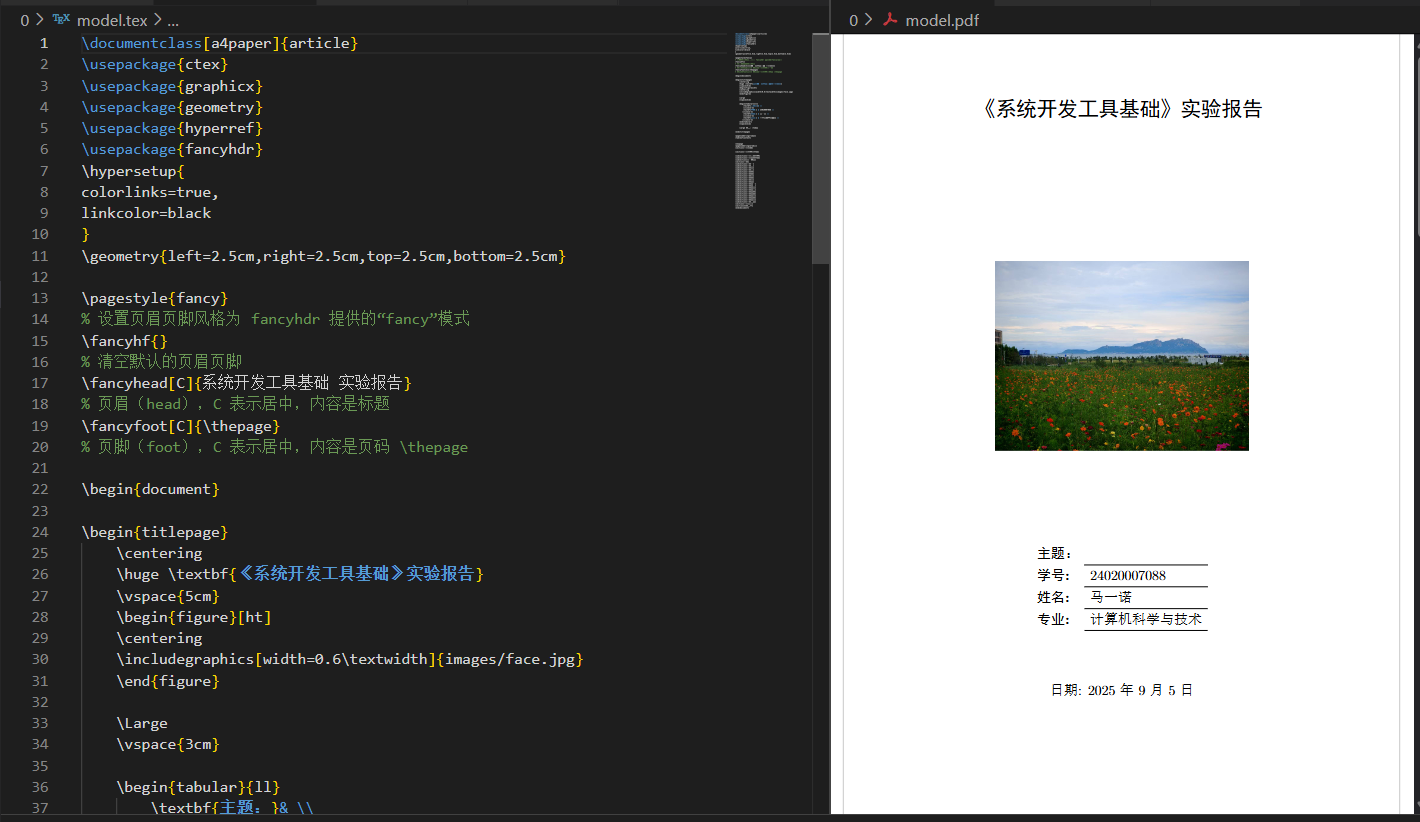
\includegraphics[width=1\textwidth]{images/model1.png}
    \caption{model1}
    \label{model1}
    \end{figure}
    \begin{figure}[H]
    \centering
    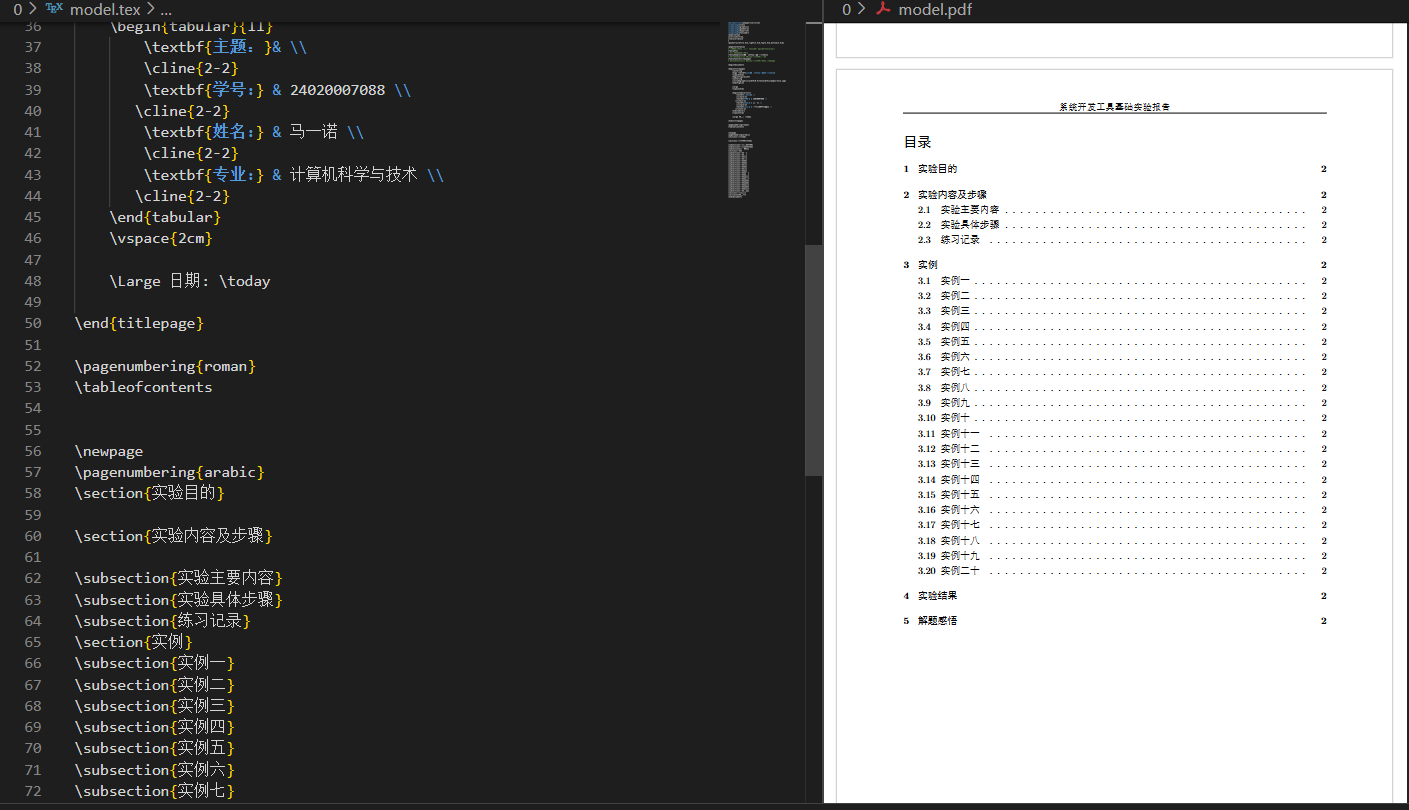
\includegraphics[width=1\textwidth]{images/model2.png}
    \caption{model2}
    \label{model2}
    \end{figure}
\section{解题感悟}
通过使用 Git 进行版本管理和 LaTeX 进行文档排版,我更深入理解了如何高效地进行团队协作与项目管理,同时提高了文档的排版质量与自动化处理能力。
\end{document}